Considereu les funcions $f(x)=-x^2+x+6$ i $g(x)=-9x+3x^2$.

\begin{apartats}

\apartat{1,25}
Calculeu l'àrea de la regió delimitada per les dues funcions.

\begin{solucio}
Punts de tall: $-x^2+x+6=-9x+3x^2\rightarrow4x^2-10x-6=0$,
\[
x=\frac{10\pm\sqrt{(-10)^2-4\cdot4\cdot(-6)}}{8}=\frac{10\pm14}{8}=3,\ -\frac12 .
\]
Comprovem la posició de cada una de les corbes: a l'interval $\left(-\frac12,3\right)$, $f(x)>g(x)$. Per tant,
\begin{align*}
A&=\int_{-\frac12}^{3}\bigl(f(x)-g(x)\bigr)\,dx=\int_{-\frac12}^{3}\Bigl(-x^2+x+6-\left(-9x+3x^2\right)\Bigr)\,dx
=\int_{-\frac12}^{3}\left(-4x^2+10x+6\right)dx\\
&=\left[-\frac43x^3+5x^2+6x\right]_{-\frac12}^{3}=(-36+45+18)-\left(\frac4{24}+\frac54-3\right)
=27-\left(-\frac{19}{12}\right)=\boxed{\frac{343}{12}\ \text{u}^2}.
\end{align*}

\textit{Pauta oficial:} 0,5 per calcular les abscisses dels punts de tall de les dues funcions, 0,25 per plantejar
l'àrea demanada com una integral definida, 0,25 pel càlcul de la primitiva i 0,25 per aplicar correctament la
regla de Barrow i donar el resultat final.
\end{solucio}

\apartat{1,25}
Trobeu l'equació de la recta tangent a la funció $f(x)$ en el punt $(-2,0)$. Representeu aquesta recta tangent i les
funcions $f(x)$ i $g(x)$ en uns mateixos eixos de coordenades.

\begin{solucio}
El pendent ve donat per la derivada de la funció: $f'(x)=-2x+1\rightarrow f'(-2)=-2(-2)+1=5$. I la recta passa
pel punt $(-2,0)$, perquè $f(-2)=0$. Així, la recta tangent serà de la forma $y=5x+n$, amb $0=5(-2)+n$, és a
dir, $n=10$: tenim $y=5x+10$.\\
Per fer la representació gràfica, observem que la recta $y=5x+10$ passa pels punts $(0,10)$ i $(-2,0)$. La gràfica
de la funció $f$ és una paràbola amb les branques cap avall i el vèrtex en el punt
$f'(x)=-2x+1=0\rightarrow x=\frac12\rightarrow\left(\frac12,\frac{25}{4}\right)$, i els punts de tall amb l'eix
d'abscisses són $(-2,0)$ i $(3,0)$, ja que $-x^2+x+6=0\rightarrow x=-2$ i $x=3$. La gràfica de la funció $g$ és una
paràbola amb les branques cap amunt i el vèrtex en el punt
$g'(x)=-9+6x=0\rightarrow x=\frac32\rightarrow\left(\frac32,-\frac{27}{4}\right)$, i els punts de tall amb l'eix
d'abscisses són $(0,0)$ i $(3,0)$, ja que $-9x+3x^2=0\rightarrow x=0$ i $x=3$.
\begin{center}
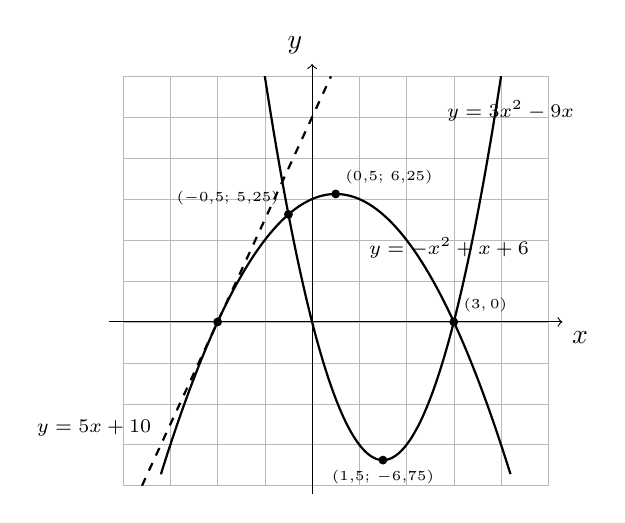
\begin{tikzpicture}[x=0.6cm,y=0.26cm]
  \draw[gray!55,very thin,xstep=1,ystep=2] (-4,-8) grid (5,12);
  \draw[->] (-4.3,0) -- (5.3,0) node[below right] {$x$};
  \draw[->] (0,-8.4) -- (0,12.6) node[above left] {$y$};
  \begin{scope}
    \clip (-4,-8) rectangle (5,12);
    \draw[\colorgrafica,thick,domain=-3.2:4.2,samples=100,smooth] plot (\x,{-(\x)*(\x)+(\x)+6});
    \draw[thick,domain=-1.4:4.4,samples=100,smooth] plot (\x,{3*(\x)*(\x)-9*(\x)});
    \draw[thick,dashed] (-3.6,-8) -- (0.4,12);
  \end{scope}
  \foreach \p in {(-0.5,5.25),(0.5,6.25),(3,0),(1.5,-6.75),(-2,0)} \fill \p circle (1.6pt);
  \node[above left,font=\tiny] at (-0.5,5.25) {$(-0{,}5;\,5{,}25)$};
  \node[above right,font=\tiny] at (0.5,6.25) {$(0{,}5;\,6{,}25)$};
  \node[above right,font=\tiny] at (3,0) {$(3,0)$};
  \node[below,font=\tiny] at (1.5,-6.75) {$(1{,}5;\,-6{,}75)$};
  \node[font=\scriptsize,\colorgrafica] at (2.9,3.6) {$y=-x^2+x+6$};
  \node[font=\scriptsize] at (4.2,10.3) {$y=3x^2-9x$};
  \node[font=\scriptsize,left] at (-3.2,-5.2) {$y=5x+10$};
\end{tikzpicture}
\end{center}

\textit{Pauta oficial:} 0,5 per l'equació de la recta tangent demanada, i 0,75 per la representació gràfica de les
tres gràfiques: 0,25 per la gràfica de la recta i 0,25 per cada una de les paràboles.
\end{solucio}

\end{apartats}
